
% IzPack - Documentation

% Custom actions

\chapter{\label{cha:customactions}Custom Actions} (by Klaus \textsc{Bartz})

\section{Overview}

In general the installation procedure is separated into several
steps. The first step, let's call it the \emph{data collection phase},
is getting specific data needed for the installation process.
Typically this is done by typing all neded data into one or more panels,
if a GUI is used, or automatically by reading the data from a config file.
In general nothing will be changed on the system until all needed data is
obtained. But mostly - depending on to the information, e.g. the
destination path - different input panels are involved.

If all needed data is collected the second step will be perfomed,
let us call it the \emph{action phase}. During this step the state of
the locale machine will be changed, e.g. files will be copied to
the installation destination or some short cuts will be registered.
Each of this subsequent steps are denoted as actions. There are actions
intended to be reused, so called common actions, and actions for one special
purpose only, so called custom actions. In IzPack there are already some
common actions, for example "file transfer", "parse" or "execute".

The third step, the \emph{reporting phase}, is normally
represented by a panel that reports the result state of the installation
(OK, or not OK) and a simple good bye message.

With IzPack there are two ways to implement custom actions. Firstly
it is always possible to define a custom panel that perfoms the desired
actions too. Secondly, and that's the new, custom actions are supported.

Panels still may be used for actions that are perfomed, e.g.
before files are transferred or after the "execute" action.
But if the needed action depends on the selected or already installed
packages, this works also, but the implementation effort is much higher.

If the action should be performed for several amount of elements of a
pack, using custom actions will be more easy than using panels.
Additional custom actions may be defined for installation, but also for
packaging and uninstallation purposes. If a custom action is also needed
for uninstallation purposes, it'll be always a good idea to implement a
corresponding installation action as custom action, but not as panel.

\section{How It Works}

Custom actions are implemented as listeners. Each listener implements
callback methods that will be called at well-defined points. The method
\texttt{InstallerListener.afterFile} for example will be called after
a file has been copied. There are different interfaces intended for being
used at packaging time, at installation time and at uninstallation time.

Each interface is implemented by a class with the prefix
"Simple" (e.g. SimpleCompilerListener) that implements all declared interface
methods with an empty body. These classes may be used as base classes
for own listener implementations.

To apply custom actions to the installer, an entry in the apropriate
install.xml file is needed. The configuration of listeners starts with
the facultative ELEMENT "listeners" which can contain one or more ELEMENTs
of "listener". For a "listener" there are three attributes which determine the
"compiler", "installer" and "uninstaller" custom action pupose.
Additionally it is possible to make the listener OS dependent using the "os"
ELEMENT.

If file related data will be set, the facultative ELEMENT
"additionaldata" is defined for the ELEMENTs "file", "singlefile"
and "fileset". This data will be automatically moved to the
corresponding PackFile objects in the install.jar. Extraction and
usage should be implemented in a install custom action (see
example).




\subsection{Custom Action Types}

Custom actions are intended to be used at packaging time, at installation time
and at uninstallation time. The interfaces are:
\begin{center}
\begin{tabular}{|l|l|}
\hline \textit{Custom action type} & \textit{Interface name} \\
\hline Packaging & com.izforge.izpack.compiler.CompilerListener \\
\hline
\hline Installation & com.izforge.izpack.installer.InstallerListener \\
\hline
\hline Uninstallation & com.izforge.izpack.uninstaller.UninstallerListener \\
\hline
\end{tabular}\
\end{center}

\subsubsection{Custom Actions At Packaging}

\paragraph{UML Diagram}

\begin{center}
\fbox{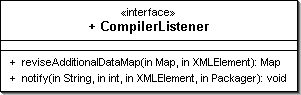
\includegraphics[scale=1.0]{img/CompilerListener}}
\end{center}\

\paragraph{Description}

\begin{itemize}

\item \textit{(constructor)} : only the default constructor will
be used. It is called from Compiler just after creating the packager.
Therefore initializing will be better during in the first \texttt{notify} call.

\item \texttt{reviseAdditionalDataMap} gives the facility to add
data to each \texttt{PackFile} object. This is the place where
file related data can be transferred from the install xml file
into the install jar file. Although each key and value of the map can be any
type, but the class definitions of all used types must therfore be contained
in the installer jar file or in the VM's classpath. In general strings
are the best choice for being used as keys or values. All keys must be
unique over all registered \texttt{CompilerListeners}. Each call of this
method adds own key value pairs to the given \texttt{existenDataMap} because
more than one listener can be used. If the given map is null, a
new one will be created.

\item \texttt{notify} is called at the beginning and at the end of each
"add" method call which is called in \texttt{Compiler.executeCompiler}.

\end{itemize}\

\subsubsection{Custom Actions At Installing Time}

\paragraph{UML Diagram}

\begin{center}
\fbox{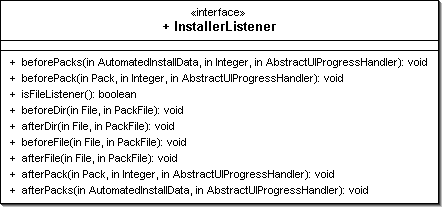
\includegraphics[scale=1.0]{img/InstallerListener}}
\end{center}\

\paragraph{Description}

\begin{itemize}

  \item \textit{(constructor)} : only the default constructor will
  be used. It is called from \texttt{Unpacker.run} before unpacking.

  \item \texttt{beforePacks} will be called each time before an unpacking
  call is performed.

  \item \texttt{beforePack} is called before a package is
  installed. Pack object and the number of the pack are passed.

  \item \texttt{isFileListener} determines whether the next four
  methods are called or not. This is a little performance optimizing.

  \item \texttt{beforeDir} is called before a directory is created.
  In this case, when file listeners exist, directories are created
  recursively and the method is called at each step. The file and the
  current \texttt{PackFile} object are passed.
  \item \texttt{afterDir} is called directly after the directory
  creation.
  \item \texttt{beforeFile} is called before a file is created. The file
  and \texttt{PackFile} object are passed as parameters.
  \item \texttt{afterFile} is the best place to perform file
  related actions. The given \texttt{PackFile} objects contains
  the additional data which was set at packaging.
  \item \texttt{afterPack} will be just called after the pack is
  closed.
  \item \texttt{afterPacks} is the last step before the handler
  will be stopped.
\end{itemize}\

\subsubsection{Custom Actions At Uninstalling Time}

\paragraph{UML Diagram}

\begin{center}
\fbox{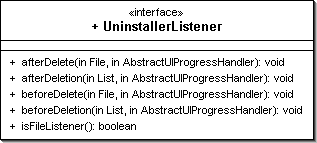
\includegraphics[scale=1.0]{img/UninstallerListener}}
\end{center}\

\paragraph{Description}

\begin{itemize}

  \item \textit{(constructor)} : only the default constructor will
  be used. It is called from \texttt{Destroyer.run} as first call.
  \item \texttt{beforeDeletion} will be called after execute files was performed.
  The given list contains all \emph{File} objects which are marked for deletion.
  \item \texttt{isFileListener} determines whether the next two
  methods are called or not.
  \item \texttt{beforeDelete} is the method which, is called before
  a single file is deleted. The \emph{File} object is given as
  parameter.
  \item \texttt{afterDelete} will be invoked after the delete call
  for a single file.
  \item \texttt{afterDeletion} is the last call before the
  cleanup of created data is performed.
\end{itemize}\

\subsection{Package Path}
Custom actions must always implement one of the given listener
interfaces. As mentioned above, it is also possible to derive from
one of the "Simple" listeners. The package path is facultative, only the
class name must be unique over all custom actions. The preparation of a
custom action for providing it with an installation is very similar to panels.
Custom actions must also be packed into a jar file with the name
of the custom action class name. This jar file should be placed in
\texttt{[IzPackRoot]/bin/customActions}, may be
\begin{verbatim}
[IzPackRoot]/bin/customActions/MyCompilerListener.jar
[IzPackRoot]/bin/customActions/MyInstallerListener.jar
[IzPackRoot]/bin/customActions/MyUninstallerListener.jar
\end{verbatim}
In the default Ant definition file (build.xml) there are some
targets for this stuff.


\subsection{Correlated Stuff}
\subsubsection{Native Libraries for Uninstallation}
If a custom action uses JNI at installation time, often the
associated uninstall custom action needs JNI too. For this
situation it is possible to declare a native library for
unstallation. The only work to do is to add a \texttt{stage}
attribute to the \texttt{native} tag in the install xml file like
\footnotesize
\begin{verbatim}
<!-- The native section. We specify here our os dependant
libs..--> <native type="3rdparty"
name="MyOSHelper.dll"stage="both" >
   <os family="windows" />
</native>
\end{verbatim}
\normalsize

The needed additional classes are packed into
lib/uninstaller-ext.jar. If a native library is defined for
uninstallation, this file will also be packed into the
installer.jar as IzPack.unistaller-ext and used at its right
position.


\section{What You Have To Do}
Follow the steps that are needed to create and use custom actions
with the "normal" source environment (not standalone compiler)
using Ant. Of course, it works also with the standalone compiler.

\subsection{\label{sec:caPackaging}Custom Actions at Packaging (CompilerListener)}

\begin{itemize}
  \item Implement \texttt{com.izforge.izpack.compiler.CompilerListener} or
  extend \texttt{com.izforge.izpack.compiler.SimpleCompilerListener}.
  Place it as \texttt{[IzPackRoot]/src/lib/[MyPackagePath]/MyCompilerListener.java}.

  \item Add a "compile.simple" antcall in to \texttt{[IzPackRoot]/src/build.xml}.
\footnotesize
\begin{verbatim}
<antcall target="compile.listener.simple">
  <param name="listener" value="MyCompilerListener"/>
  <param name="listener-dir" value="MyCompilerListener"/>
  <param name="listener-include" value="[MyPackagePath]"/>
</antcall>
\end{verbatim}
\normalsize

  \item Run \texttt{[IzPackRoot]/src/build.xml}.

  \item Add a "listeners" ELEMENT with a "listener" ELEMENT with
  a "compiler" attribute in to [MyProjectPath]/install.xml
\footnotesize
\begin{verbatim}
  <listeners>
    <listener compiler="MyCompilerListener" />
  <listeners>
\end{verbatim}
\normalsize

  \item Compile with
\footnotesize
\begin{verbatim}
java -jar [IzPackRoot]/lib/compiler.jar -HOME [IzPackRoot]
  [MyProjectPath]/install.xml -b [MyProductPath] -o
  [MyBuildPath]/install.jar
\end{verbatim}
\normalsize

  \item Test it
\end{itemize}\

\subsection{Custom Actions at Installation Time (InstallerListener)}
Perform the same steps as described in \ref{sec:caPackaging}, replace
all occurrences of "CompilerListener" with "InstallerListener" and
"compiler" with "installer".

\subsection{Custom Actions at Uninstallation Time
(UninstallerListener)} Perform the same steps as described in
\ref{sec:caPackaging}, replace all occurrences of
"CompilerListener" with "UninstallerListener"and "compiler" with
"uninstaller".

\section{Example}
Let us say, we want to set access rights for files and directories
on Unix. The Java sources are placed in the directory \\
\texttt{[IzPackRoot]/sample/src/com/myCompany/tools/install/listener}.
There are the files ChmodCompilerListener.java and
ChmodInstallerListener.java.
\begin{itemize}
  \item Copy the files too
  [IzPackRoot]/src/lib/com/myCompany/tools/install/listener
  \item In [IzPackRoot]/src/build.xml there are the lines
\footnotesize
\begin{verbatim}
    <!-- CUSTOM ACTION test START
    CUSTOM ACTION test END -->
\end{verbatim}
\normalsize Uncomment them (activate the lines between them).
  \item Build IzPack new.
  \item Compile a test installation with
\footnotesize
\begin{verbatim}
java -jar [IzPackRoot]/lib/compiler.jar -HOME [IzPackRoot]
  [IzPackRoot]/sample/listener/install.xml
  -b [IzPackRoot]/sample/listener -o
  [IzPackRoot]/sample/listener/install.jar
\end{verbatim}
\normalsize
  \item Install it
\footnotesize
\begin{verbatim}
java -jar install.jar
\end{verbatim}
\normalsize
\end{itemize}\
